\documentclass[]{article}

%opening
\title{Quantum teleportation protocol}
\author{Emilio Peláez}

\usepackage[margin=1.0in]{geometry}
\usepackage{braket}
\usepackage{physics}
\usepackage{amsmath}
\usepackage{graphicx}
\usepackage{mathtools}
\usepackage[colorlinks]{hyperref} 

\newcommand\Hto{\xrightarrow{H}}
\newcommand\Xto{\xrightarrow{X}}
\newcommand\Zto{\xrightarrow{Z}}
\newcommand\Htopsi{\xrightarrow{H\ket{\psi}}}
\newcommand\Rzto{\xrightarrow{R_z}}
\newcommand\Cnot{\xrightarrow{CNOT\ket{\psi\phi}}}

\begin{document}

\maketitle

\begin{abstract}
	Equations typed in \LaTeX\ to explain quantum teleportation protocol implemented with Qiskit in python. Complete description available \href{https://github.com/epelaaez/QuantumLibrary/tree/master/algorithms/teleportation}{here}.
\end{abstract}

\section*{Equations}
We define three states $\ket{\psi}$, $\ket{\phi}$, and $\ket{\omega}$. $\ket{\psi}$ will be the state we want to send, $\ket{\phi}$ will be an ancillary qubit, and $\ket{\omega}$ will be the qubit to which we want to send the state originally in $\ket{\psi}$. To summarize:

\begin{equation}
    \ket{\psi}\textrm{: sender qubit, }\ket{\phi}\textrm{: ancillary qubit, }\ket{\omega}\textrm{: receiver qubit.}
\end{equation}

This is the circuit we are going to describe with equations in this paper:

\begin{figure}[h!] 
    \centering
    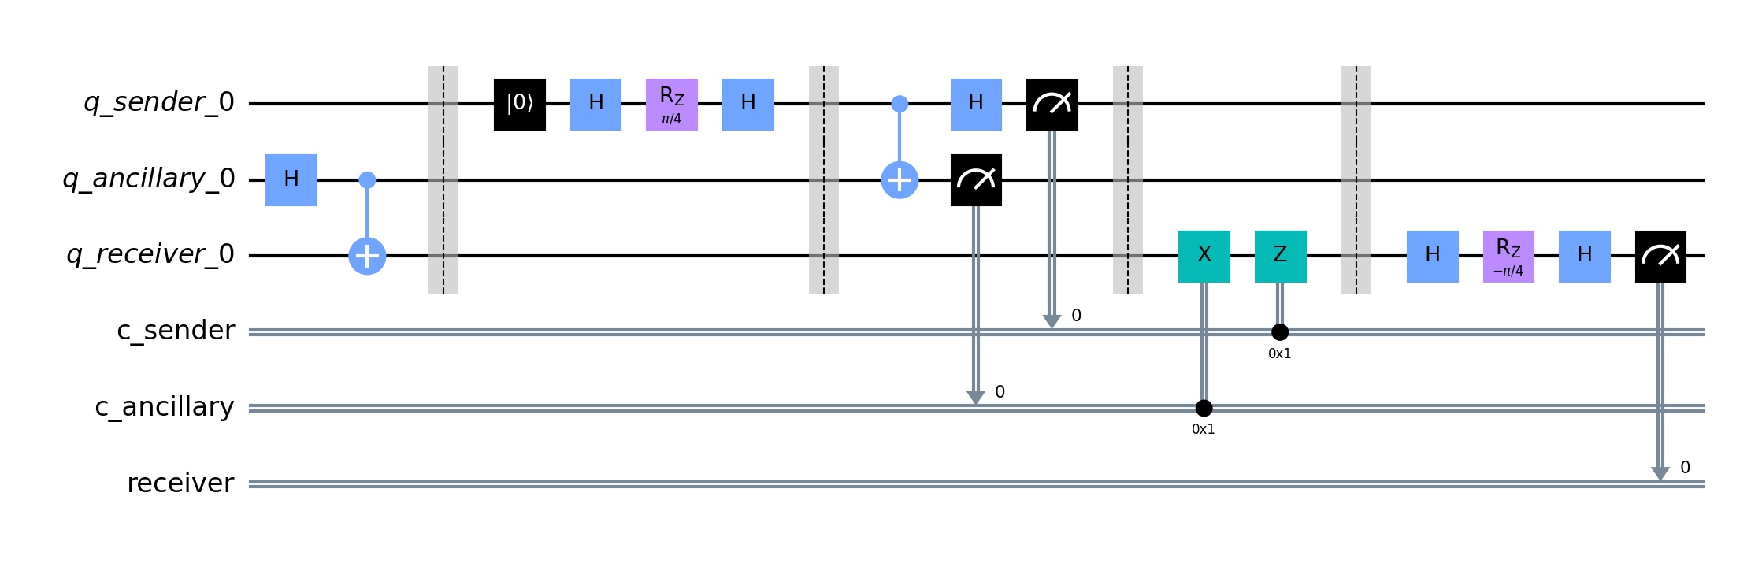
\includegraphics[scale=0.4]{images/qtp-converted.pdf}
    \caption{Quantum teleportation protocol circuit}
    \label{fig:qtp_circuit}
\end{figure}

As you can see, the first thing we do is entangle $\ket{\phi}$ with $\ket{\omega}$. This gives us the state:

\begin{equation} \label{first_entanglement}
    \ket{\psi} \otimes \frac{1}{\sqrt{2}}(\ket{00} + \ket{11})
\end{equation}

Note that in this equation and onward, we will describe our state as $\ket{\psi\phi\omega}$. For example, the state $\ket{010}$ means that $\ket{\psi} = \ket{0}$, $\ket{\phi} = \ket{1}$, and $\ket{\omega} = \ket{0}$. After entangling $\ket{\phi}$ and $\ket{\omega}$, we prepare $\ket{\psi}$ to the state we want to send. Let's now focus on this state and how it will result after applying the corresponding gates. 

\begin{align}
    \ket{\psi} = \ket{0} &\Hto \frac{1}{\sqrt{2}}(\ket{0} + \ket{1}) \\
    &\Rzto{}  \frac{1}{\sqrt{2}}\left(e^{-i\frac{\pi}{8}}\ket{0} + e^{i\frac{\pi}{8}}\ket{1}\right) \\ 
    &\Hto{} \frac{1}{2}\left(e^{-i\frac{\pi}{8}}(\ket{0} + \ket{1}) + e^{i\frac{\pi}{8}}(\ket{0}-\ket{1})\right) = \cos{\frac{\pi}{8}}\ket{0} - \sin{\frac{\pi}{8}}\ket{1} \label{prepare_send_state}
\end{align}

The simplified state at \eqref{prepare_send_state} is the one we will be sending to $\ket{\omega}$. Now, we are going to entangle $\ket{\psi}$ with $\ket{\phi}$ using a CNOT gate and then we are going to send $\ket{\psi}$ through a Hadamard gate. Before applying any gates, let's see our state up to here. We can found this state by replacing $\ket{\psi}$ in \eqref{first_entanglement} with the state for $\ket{\psi}$ we got in \eqref{prepare_send_state}. 

\begin{align} \label{expanded_state}
    \left(\cos{\frac{\pi}{8}}\ket{0} - \sin{\frac{\pi}{8}}\ket{1}\right) \otimes \frac{1}{\sqrt{2}}\left(\ket{00} + \ket{11}\right) = \frac{1}{\sqrt{2}}\left(\cos{\frac{\pi}{8}}(\ket{000} + \ket{011}) - \sin{\frac{\pi}{8}}(\ket{100} + \ket{111})\right)
\end{align}

First we are going to send our state through the CNOT gate, where $\ket{\psi}$ acts as the control qubit and $\ket{\phi}$ as the target qubit, and then we are going to send $\ket{\psi}$ through a Hadamard gate. The following equations describe this operations. For simplicity, we will denote the state we are starting with as $\ket{\psi\phi\omega}$, this state is the one we ended up with in \eqref{expanded_state}.

\begin{align}
     \ket{\psi\phi\omega} &\Cnot{} \frac{1}{\sqrt{2}}\left(\cos{\frac{\pi}{8}}(\ket{000} + \ket{011}) - \sin{\frac{\pi}{8}}(\ket{110} + \ket{101})\right) \\ 
     &\Htopsi{} \frac{1}{2}\left(\cos{\frac{\pi}{8}} (\ket{000} + \ket{100} + \ket{011} + \ket{111}) - \sin{\frac{\pi}{8}}(\ket{010} - \ket{110} + \ket{001} - \ket{101}) \right) \label{before_measuring}
\end{align}

Here it gets a little bit tricky, since we are going to measure $\ket{\psi}$ and $\ket{\phi}$. As you may know, there are 4 possible states we might end up with, these are $\ket{00}$, $\ket{01}$, $\ket{10}$ and $\ket{11}$. And for each of this four states, you can have either $\ket{0}$ or $\ket{1}$ for our last qubit: $\ket{\omega}$. This gives us the 8 possible states we can see in \eqref{before_measuring}. Since we are only going to measure the first two qubits, $\ket{\omega}$ will remain in a superposition of states, we will examine the 4 possibilities in the following equations:

\begin{align}
    \textrm{When} \ket{\psi\phi}=\ket{00} \textrm{, } \ket{\omega}&=\cos{\frac{\pi}{8}}\ket{0} - \sin{\frac{\pi}{8}}\ket{1} \\
    \textrm{When} \ket{\psi\phi}=\ket{01} \textrm{, } \ket{\omega}&=-\sin{\frac{\pi}{8}}\ket{0} + \cos{\frac{\pi}{8}}\ket{1} \\
    \textrm{When} \ket{\psi\phi}=\ket{10} \textrm{, } \ket{\omega}&=\cos{\frac{\pi}{8}}\ket{0} + \sin{\frac{\pi}{8}}\ket{1} \\
    \textrm{When} \ket{\psi\phi}=\ket{11} \textrm{, } \ket{\omega}&=\sin{\frac{\pi}{8}}\ket{0} + \cos{\frac{\pi}{8}}\ket{1}
\end{align}

Now, as you can see in the circuit, we are going to send $\ket{\omega}$ through some gates depending on the measurements we made. We are going to apply a Pauli-X gate if $\ket{\phi} = \ket{1}$, followed by a Pauli-Z gate if $\ket{\psi}=\ket{1}$. After applying this conditional gates, $\ket{\omega}$ should be in the state of $\ket{\psi}$ showed in \eqref{prepare_send_state}, meaning that the teleportation was completed successfully. Let's see what happens exactly in each case, we will start with the case in which $\ket{\psi\phi}=\ket{00}$. Well, in this case no further gate is applied, we just have the following state.

\begin{equation} \label{first_case}
    \ket{\omega} = \cos{\frac{\pi}{8}}\ket{0} - \sin{\frac{\pi}{8}}\ket{1}
\end{equation}

Now, let's look at what happens when $\ket{\psi\phi}=\ket{01}$. We will only apply a Pauli-X gate. 

\begin{align} \label{second_case}
    \ket{\omega}=-\sin{\frac{\pi}{8}}\ket{0} + \cos{\frac{\pi}{8}}\ket{1} \Xto{} \cos{\frac{\pi}{8}}\ket{0} - \sin{\frac{\pi}{8}}\ket{1}
\end{align}

Now, we look at the case where $\ket{\psi\phi}=\ket{10}$. In this case, we only apply a Pauli-Z gate. 

\begin{align} \label{third_case}
    \ket{\omega}=\ket{\omega}&=\cos{\frac{\pi}{8}}\ket{0} + \sin{\frac{\pi}{8}}\ket{1} \Zto{} \cos{\frac{\pi}{8}}\ket{0} - \sin{\frac{\pi}{8}}\ket{1}
\end{align}

Finally, we look at what happens when $\ket{\psi\phi}=\ket{11}$. This time, we apply a Pauli-X gate followed by a Pauli-Z gate.

\begin{align} 
    \ket{\omega}=\sin{\frac{\pi}{8}}\ket{0} + \cos{\frac{\pi}{8}}\ket{1} &\Xto{} \cos{\frac{\pi}{8}}\ket{0} + \sin{\frac{\pi}{8}}\ket{1} \\
    &\Zto{} \cos{\frac{\pi}{8}}\ket{0} - \sin{\frac{\pi}{8}}\ket{1} \label{fourth_case}
\end{align}

At this point, the quantum teleportation protocol is over. $\ket{\omega}$ is in the state we showed on \eqref{prepare_send_state}, meaning that we successfully sent the state from $\ket{\psi}$ into $\ket{\omega}$. To achieve this, we needed to send two bits of information through classical channels, which allowed us to perform the controlled operations showed in \eqref{first_case}, \eqref{second_case}, \eqref{third_case}, and \eqref{fourth_case}. It is common to think that this use of classical channels throws away the whole purpose of teleporting a quantum state, but it really doesn't. This classical communication is really the only way of ensuring that we teleport the state successfully; if we didn't apply this step, we would be stuck with one of the four possibilities shown above without the person that has $\ket{\omega}$ having a clue about what $\ket{\psi\phi}$ is, therefore this person would only have the intended state $1/4$ of the time.

In the circuit shown in figure \ref{fig:qtp_circuit}, we apply some additional gates to $\ket{\omega}$. This is just a way to ensure that the teleportation protocol was successful when running in IBM's quantum computers. As you can see, this gates are the same that were applied to the state $\ket{\psi}$ when preparing it, but backwards (which turns out to be the same in this case). As you may know, quantum computation is reversible, so performing this operations will turn $\ket{\omega}$ back to the state $\ket{0}$ (we are applying the operations shown in \eqref{prepare_send_state} but in reverse). This makes it easier to measure if the protocol was successful since the computer will measure $\ket{\omega}$ to be $\ket{0}$ with certainty (without taking into account noise of actual quantum hardware). 

\end{document}